\documentclass[12pt]{article}
\usepackage[UKenglish]{babel} 
\usepackage{alphalph,cite}
\usepackage{amsmath}
\usepackage{amsfonts}
\usepackage{graphicx,caption}
\usepackage{floatrow}
\usepackage{xcolor}
\usepackage{tabularx,booktabs}
\usepackage{wrapfig}
\usepackage{array}
\usepackage{float}
\usepackage{geometry}
\usepackage{listings}
\usepackage[doublespacing]{setspace}
\captionsetup{width=0.8\textwidth}
\newcommand{\Int}{\int\limits}
\geometry{
 a4paper,
 total={170mm,257mm},
 left=30mm,
 right=20mm,
 top=20mm,
 }
 \pagestyle{headings}
\title{Slice reconstruction from projections}
\begin{document}
\maketitle

\clearpage
\setcounter{page}{2}                    % make it start with "ii"
\tableofcontents 
\clearpage       
\section{Introduction}
Being a football player, I have experienced a multitude of injuries in my life. Whenever I was hurt I went to the doctor who would examine if any bones or tissue were damaged. I underwent medical scans such as X-ray and CT scans, which created images of my internal structure, such that my injury could be diagnosed without any surgical interventions. I was fascinated by the technology, which lead me to inquire into the processes driving the mechanisms behind such medical equipment. From physics class I already comprehended the fundamental concepts of an X-ray scan. The X-ray machine directs the rays toward the part of the body that is being examined. When the X-rays come into contact with body tissue they produce an image on a metal film. Soft tissues such as skin and organs are unable to absorb the high-energy rays, hence, they pass through the tissue. However, the bones in our body are relatively dense in comparison and are able to absorb at least parts of the radiation. The X-ray film than develops an image based on which areas were exposed to the X-rays. This reveals that the function of the basic X-ray machine is mostly integrated into the field of physics. However, when researching about CT scans, the processes becomes more interesting in a mathematical sense.

The term CT refers to "computer tomography" and is an specialised X-ray imaging procedure. Unlike conventional X-ray machines, the CT scanner employs a motorised X-ray source that rotates around the circular opening of the machine in which the patient is located. The source is quickly rotated around the body, these X-rays are then picked up by detectors after they have passed through the body and are transmitted to a computer. The detector only records the intensity of the X-rays as they leave the patient, it does not directly illustrate the inner structure. Once the X-ray has completed one full rotation, the computer employs mathematical techniques to construct a 2D cross-sectional image of the structure. 

Figure 1 illustrates the basic scheme of a CT scanner. The source emits parallel X-rays at increments of around 1 to 9 millimetres through the patient which are received by the detector. This is done at some $n$ number of angles $\theta$ in a full rotation.
\begin{figure}[hbt]
	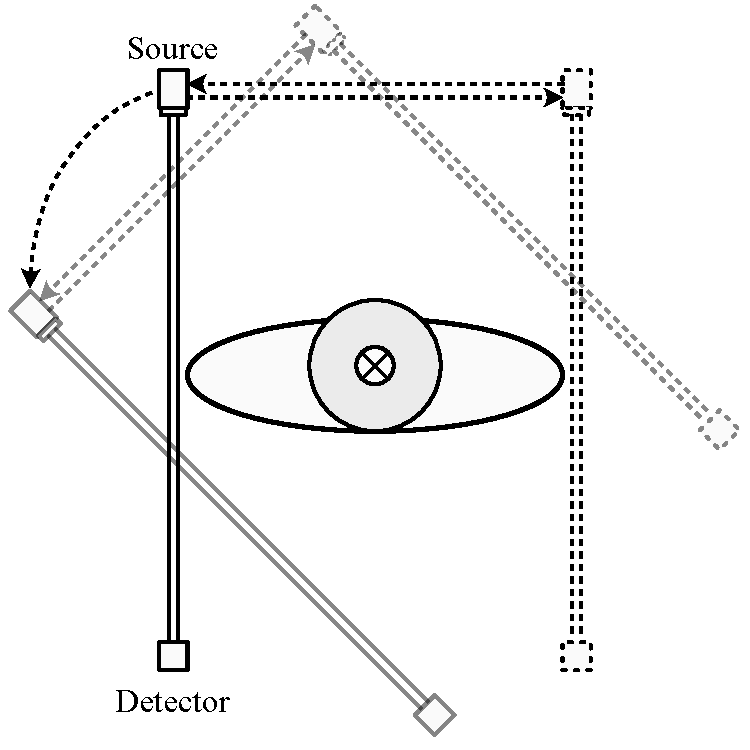
\includegraphics[width=.4\textwidth]{images/ct_scanner.pdf}	
	\caption{Illustration of the computer tomography (CT) procedure. An X-ray source is shifted along the arrow direction for a given angle $\theta$ such that the X-ray pass the patient and are detected by an X-ray detector. For a given angle, this will result in 1-dimensional intensity distribution for the given angle. Taking multiple intensity distributions delivers a whole sinogram, which is analysed by the inverse Radon transform to reconstruct the 3-dimensional distribution of material coefficients in the body.}
\end{figure}
So at every of the $n$ angles the CT scanner records a number of discrete points with an assigned intensity. The intensity that is detected by the sensor is dependent on the attenuation coefficient and width of the material the X-ray passes through. The recorded final intensities then provide us with enough information to reconstruct the object. The understanding and investigation of the reconstruction process is the aim of this paper.
\section{Theory}
\subsection{Mathematical Model for X-Ray Tomography}
As mentioned above, one of the applications of image reconstruction is the computer tomography by X-rays. In this application the X-rays transmitted through the body are attenuated due to absorption processes. Different regions (bones, muscle, fat) in the body thereby absorb the X-ray radiation differently.  This inhomogeneous distribution of absorbing material needs to be reconstructed from CT. To relate the mathematical study following below to that application I first describe the attenuation process. 
I assume that an X-ray of an intensity $I_{0}$ is incident on a body. The X-ray is transmitted through the body without deflection and then hits a detector where its intensity is measured. Along its path through the material, a part of the radiation is absorbed. If $x$ denotes the coordinate along the path, then the different materials can be characterised by an attenuation coefficient $\mu(x)$. 
\begin{figure}[hbt]\label{fig.2}
	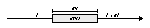
\includegraphics[width = .6\textwidth]{theory/beer_lambert_law}
	\caption{Sketch of the conditions used to derive the Beer-Lambert Law. An intensity $I$ hits a small volume element of length $dx$ and an attenuation coefficient $\mu(x)$ of the sample. After going through the sample, the intensity has changed due to absorption processes by an amount of $dI$.}
\end{figure}
The intensity change $dI$ along an infinitesimally small element $dx$ (see Figure 2) along the path can then be described by

\begin{equation}\label{eq.1}
	\frac{dI}{dx} = -I\mu(x)
\end{equation}

where the negative sign on the right side denotes that the intensity is getting smaller due to absorption processes. This first order differential equation can be solved readily by separation of variables and integration. Separation of variables yields

\begin{equation}\label{eq.2}
\frac{dI}{I}=-\mu(x)dx
\end{equation}	
and the integration results in
\begin{equation}\label{eq.3}
	\ln(I)=-\int_{0}^{x} \mu(x)dx +C
\end{equation}
where $C$ is an integration constant determined by the boundary condition required to solve the differential equation. This equation can be further transformed into
\begin{equation}\label{eq.4}
I(x)=Ae^{-\int_{0}^{x} \mu(x)dx}	
\end{equation}
with $A=e^{C}$. Assuming that the X-ray had an intensity of $I(x=0)=I_{0}$ at the beginning of the path, i.e. at $x=0$ I finally find $A=I_{0}$ and thus
\begin{equation}\label{eq.5}
I(x)=I_{0}e^{-\int_{0}^{x} \mu(x)dx}	
\end{equation}

This equation is known in physics as Lambert-Beers Law describing the attenuation of beams of radiation or particles when traversing through materials. Taking the logarithm on both sides modifies eq. \ref{eq.5} such that 

\begin{equation}\label{eq.6}
	\ln\left (\frac{I_{0}}{I(x)}\right )=\int_{0}^{x}\mu(x)dx
\end{equation}

This value is the quantity which is observed in a computer tomography experiment. It represents the cumulative effect of the local attenuation coefficient $\mu(x)$ along the path of the X-ray. From this intensity value $I(x)$, however, no information on variation of $\mu(x)$ can be obtained. In the following, I will therefore highlight the mathematical tools of how to extract the variation of the attenuation coefficient in space from a series of projections. We will generalise the description such that the attenuation coefficient is a two dimensional function, i.e. $\mu(x,y)$ which is in the following denoted by $f(x,y)=\mu(x,y)$.

\subsection{New coordinate system}
To explore the projection a 2-dimensional slice of an inhomogeneous material by X-rays into a 1-dimensional distribution it is useful to introduce a new coordinate system. In medical imaging the following new coordinate system is considered (Fig. \ref{fig.1}).
\begin{figure}[hbt]
	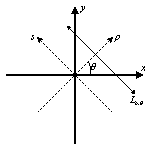
\includegraphics[width=.4\textwidth]{theory/new_coordinate_system}
	\caption{Coordinate system used in the Radon transform process. }	\label{fig.1}
\end{figure}
The new coordinate system is given by three parameters, the angle $\theta$, the distance from the origin $\rho$ and the position along the ray $L_{\rho,\theta}$ denoted by $s$. This new coordinate system is related to the cartesian coordinates $x, y$ by 
\begin{align}
 	x=\rho\cos{\theta} - s\sin{\theta}\label{eq.7}\\
 	y= \rho\sin{\theta} + s\cos{\theta}\label{eq.8}
\end{align}
The continuous set of points that form line $L_{\rho,\theta}$ can be described by eq. \ref{eq.7} and eq. \ref{eq.8}. I can also establish the normal form of the line in terms of $\rho$ as
\begin{equation}\label{eq.9}
	\rho = x\cos{\theta} + y\sin{\theta}
\end{equation}
This new coordinate system will offer to be valuable when describing lines in the following sections and presents us with the necessary information to introduce some mathematical methods that will be the core for our solving of the attenuation coefficients, in the original object.

\subsection{Radon Transform}
The Radon Transform is a mathematical transformation for computing a set of projections from a two dimensional distribution $f(x,y)$. In the context of medical imaging,$f(x,y)$ represents the slice of the body through which the X-rays are transmitted. Within the slice multiple structures with different attenuation coefficients are contained.Therefore, $f$ is a function that corresponds to the two dimensional distribution of these attenuation coefficients throughout the slice of the body. Hence, the Radon transform is the mathematical model that describes the process of our CT scan. In the following, I will denote $f(x,y)$ as a slice. The Radon transform is mathematically indicated as
\begin{equation}\label{eq.10}
	\breve{f}(\rho, \theta)= \int\limits_{\mathbb{R}} f(x,y)\, ds
\end{equation}
Eq. \ref{eq.10} illustrates that we are able to compute the projection of a slice under a certain angle $\theta$ and a distance from the origin $\rho$. The Radon transform takes the line integral along line $L_{\rho, \theta}$, which sums the attenuation coefficients along the line to calculate this projection of the slice. This is repeated for all $\theta \in [0, \pi]$ and for all $\rho \in \mathbb{R}$. In the real world, we can only measure the projection for a discrete set of $\theta$ and $\rho$, however, I  assume a continuous set for analyzing the mathematical procedures. The principle of the Radon transform for one angle is illustrated by Figure 4.
\begin{figure}[hbt]
	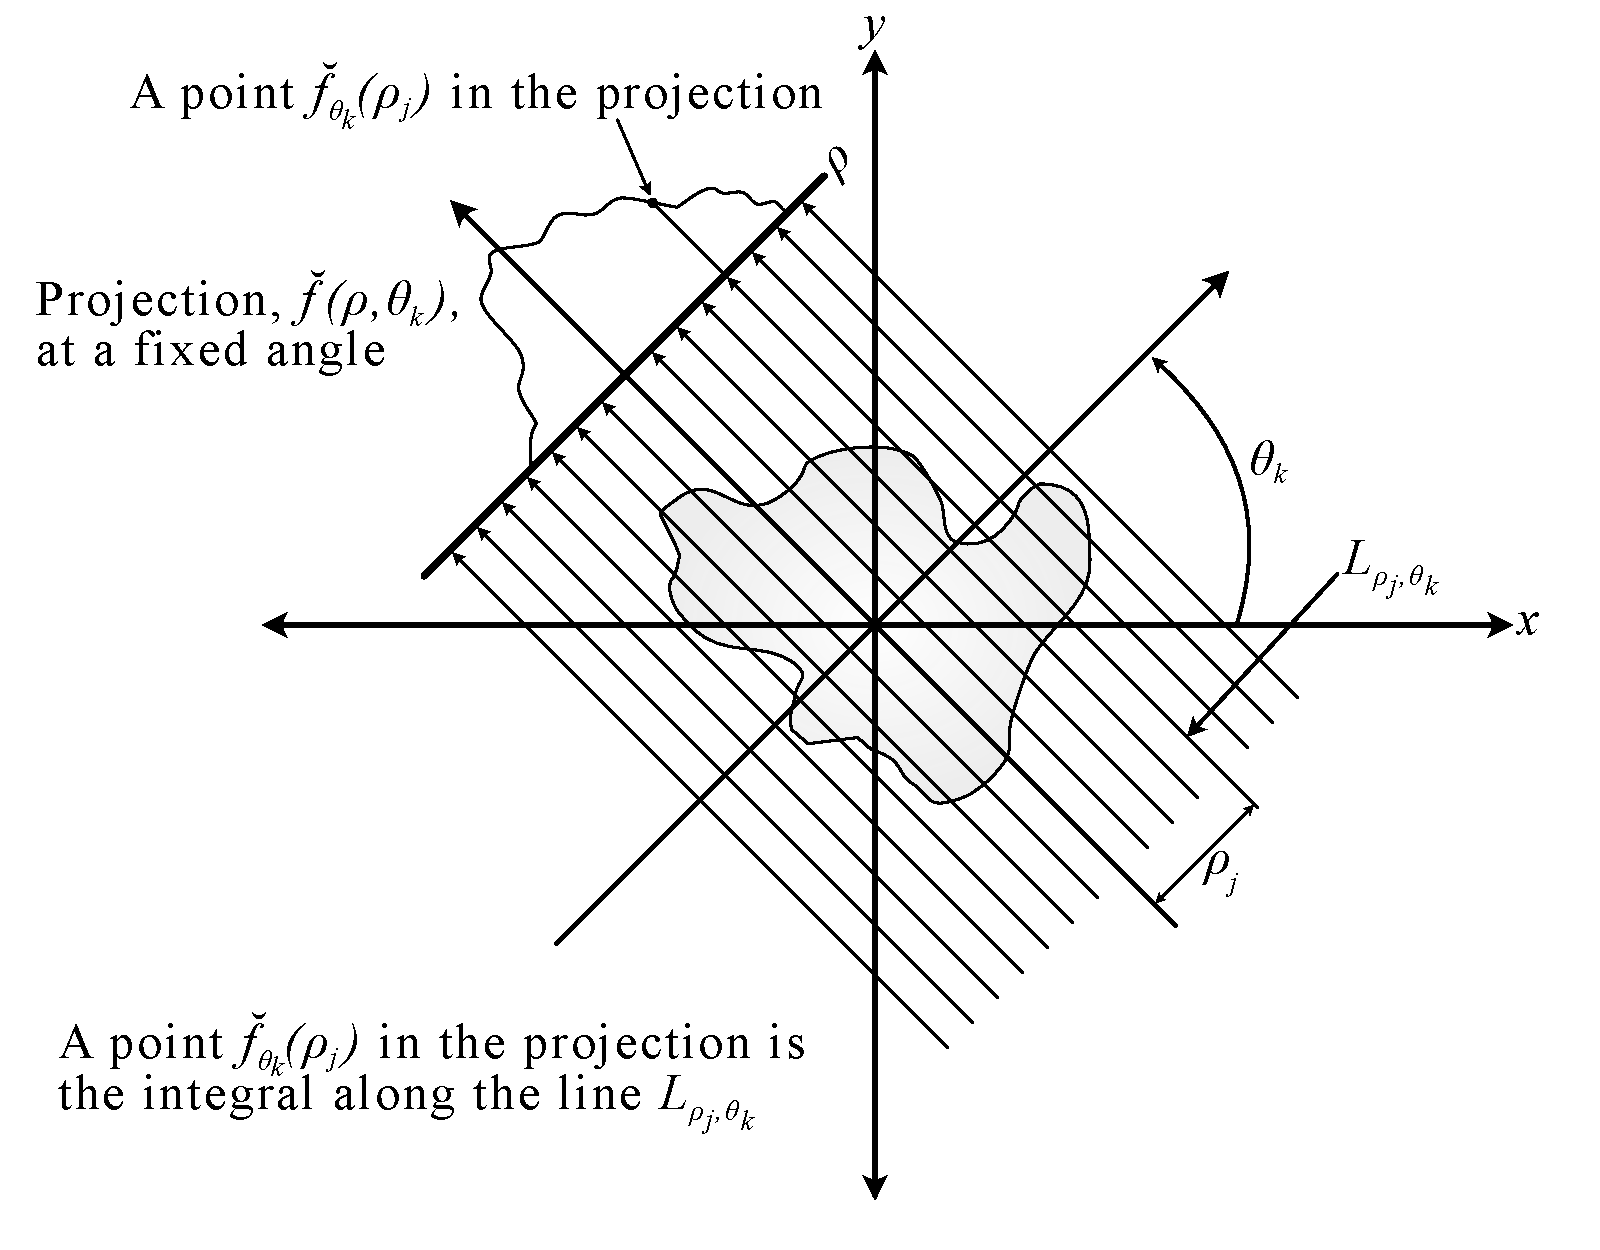
\includegraphics[width= .7\textwidth]{theory/euclidean_radon_space}
	\caption{Principle of the radon transform. The Radon transform projects a 2-dimensional distribution into a 1-dimension function for each angle of irradiation $\theta$. This set of 1-dimensional intensity distributions is then inverted by the inverse of the Radon transform.}
\end{figure}
If the Radon transform is applied along all angles $\theta$ I obtain a so-called sinogram, which is a commonly used name in medical imaging for $\breve{f}(\rho, \theta)$. Figure 5 shows an example of a slice and its corresponding sinogram, which was acquired by performing the Radon transform through a python program.
\begin{figure}[hbt]
	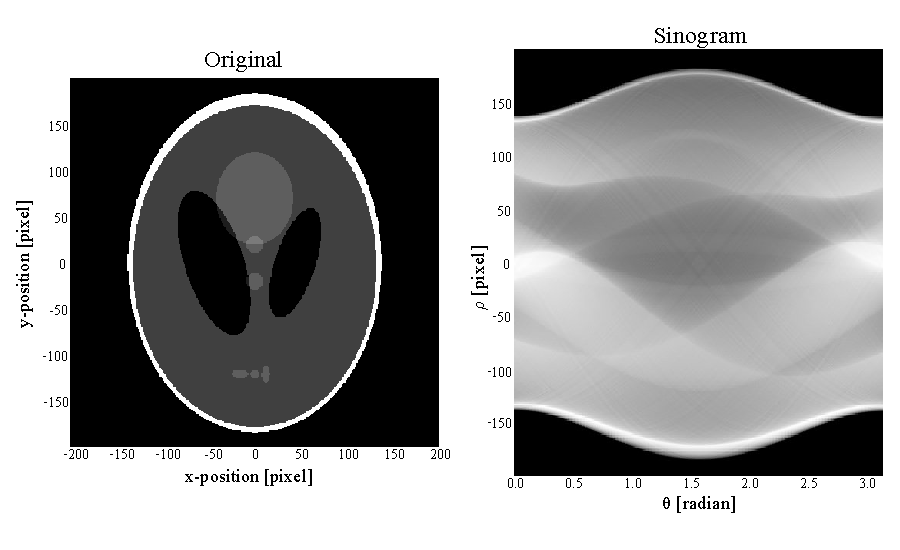
\includegraphics[width = .7\textwidth]{theory/sinogram}
	\caption{Original slice ("Shepp-Logan Phantom" [9]) and sinogram of the slice for the interval $\theta \in [0, \pi]$.}
\end{figure}
In an CT application the initial distribution of attenuation coefficients in the slice is unknown and it is the goal of the mathematical procedure to find a formula that inverts the Radon transform, such that I can reconstruct the original slice. To do so I will introduce another more explicit form of the Radon transform by substituting for $x$ and $y$ employing  eq. \ref{eq.8} and eq. \ref{eq.9}. 
\begin{equation}\label{eq.11}
	\breve{f}(\rho, \theta)=\int\limits_{\mathbb{R}} f(\rho\cos{\theta}	 - s\sin{\theta},\rho\sin{\theta} + s\cos{\theta}) \, ds. 
\end{equation}
In the following section I will employ both forms of the Radon transform interchangeably based on which best suits my needs.

\subsection{Inverse Radon Transfrom}
I have obtained a mathematical transformation for computing the projection of a slice, with a 2-dimensional distribution of attenuation coefficients $f(x,y)$. Subsequently, I will commence to investigate the inverse transform, namely to reconstruct the slice from its projections. Unfortunately, there is no single or straightforward solution to the reconstruction of the original slice. I will investigate what I call the 'smearing' back-projection and the filtered back-projection. For the filtered back-projection I will have to delve into some more advanced mathematics to obtain the desired inversion formula.
\subsubsection{'Smearing' Back-projection}
The 'smearing' back-projection is the simpler method of reconstruction a slice from its projections. It also has the benefit that is much more intuitive then the filtered back-projection and presents itself as comprehensible through illustrations. In non-mathematical terms it can be described as taking the projection at an angle $\theta$ and 'smearing' it back onto the plane of the slice. If we 'smear' the projection at only a few $\theta$ the reconstruction of even simple slices will be incredibly inaccurate. 
\begin{figure}[hbt]
	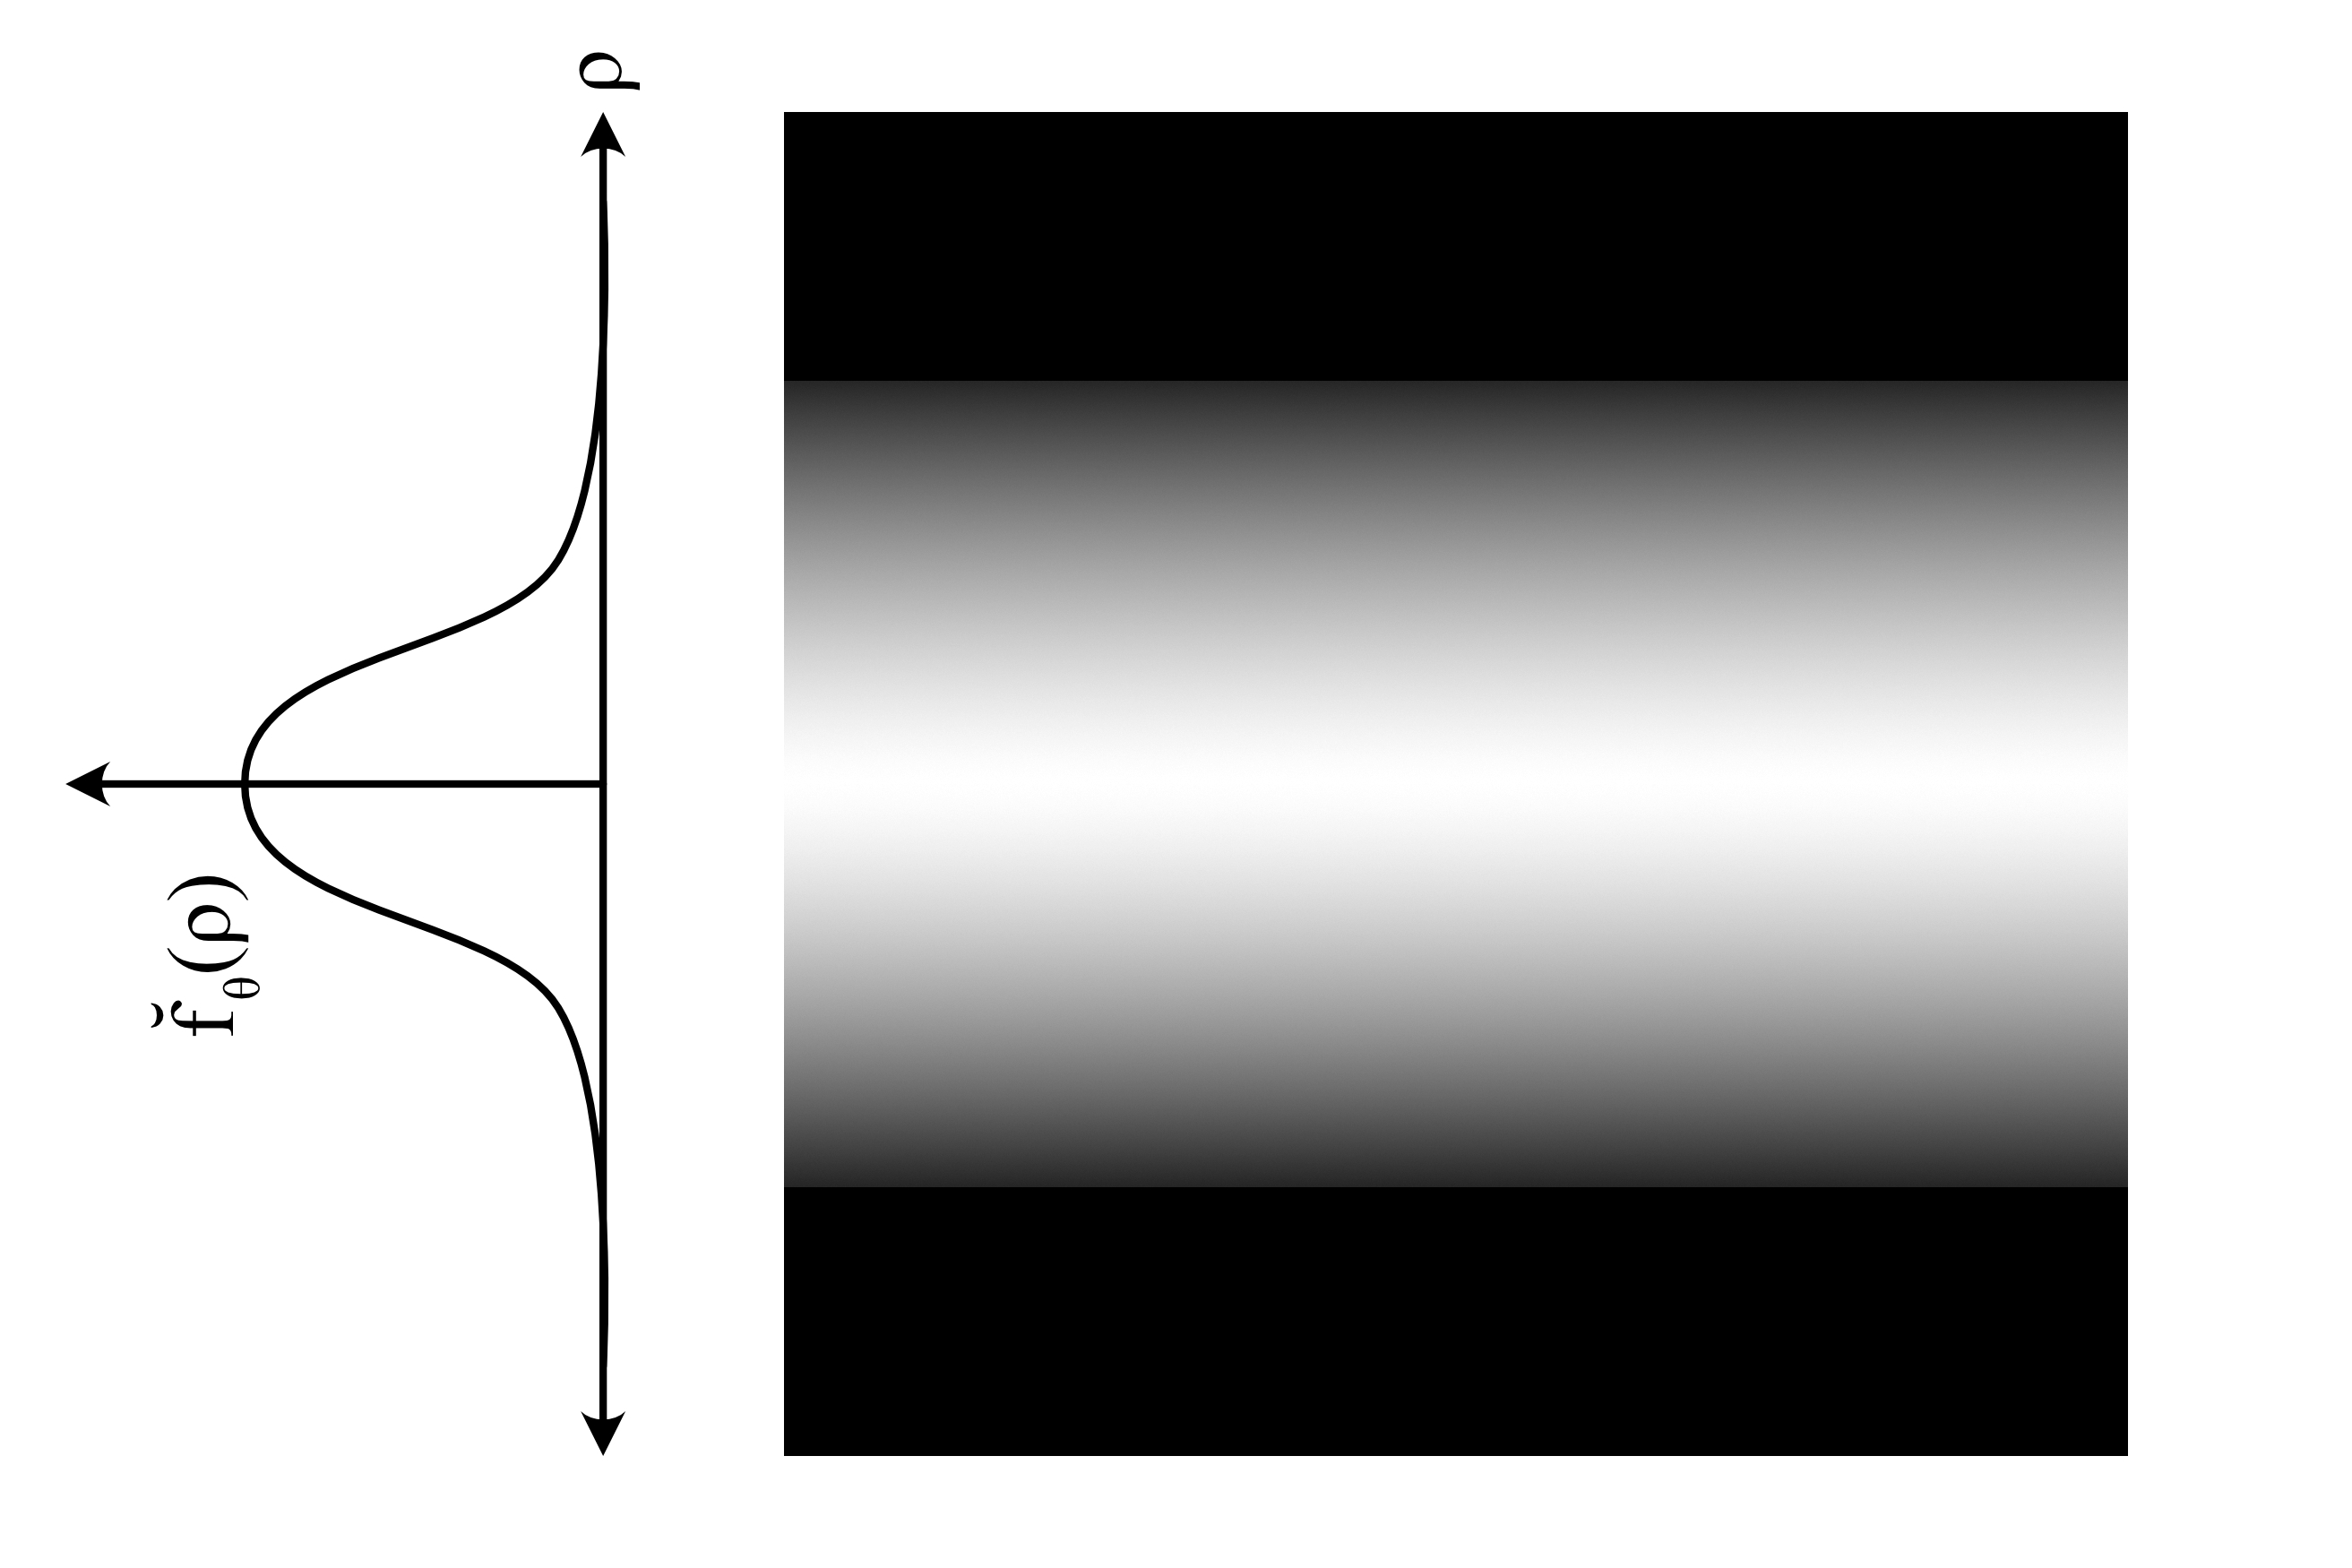
\includegraphics[width = .5\textwidth ]{inverse_radon/backprojection_smearing}
	\caption{Visualisation of 'smearing' back-projection method. The intensity distribution is smeared along the horizontal direction ($\theta~=~0$) across the image on the right.}
\end{figure}
However, If we 'smear' more projections at different $\theta$ we will have a better reconstruction of the original slice, although, there is a strong blurring in the recreated slice. This is shown in Figure 7, when I reconstructed a slice of a homogenous circle.  
\begin{figure}[hbt]
	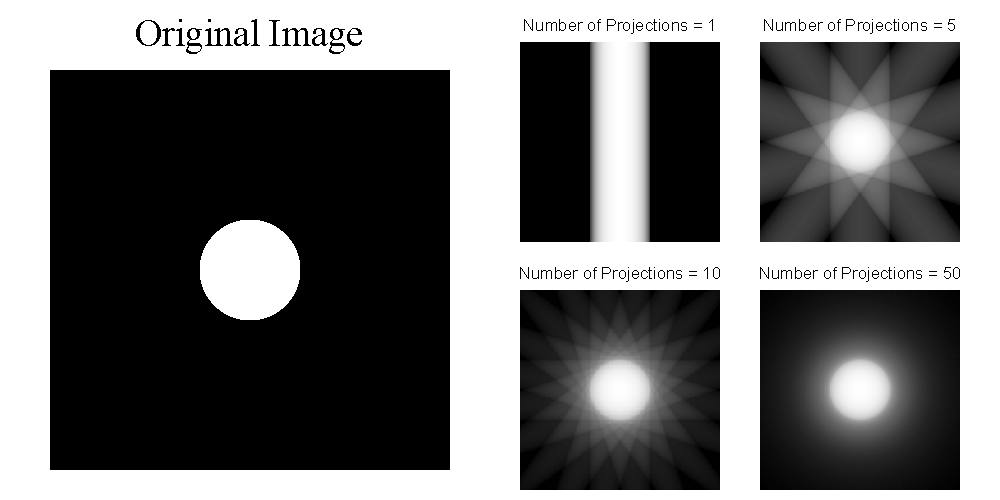
\includegraphics[width = \textwidth]{inverse_radon/smearing}
	\caption{Reconstruction with different number of projections for $\theta \in [0, \pi]$}
\end{figure}
I observe that even at 50 back-projections, although the circle is clearly noticeable, there is blurring in the reconstructed slice. It is important to note here that for the reconstruction of the slice only projections at $\theta \in [0, \pi]$ are needed, since any projection for $\theta \in (\pi, 2\pi]$ does not contain any new information and is therefore unnecessary.
I define the back-projection formula for the Radon transform mathematically as follows,
\begin{equation}\label{eq.12}
	\mathcal{B}\{\breve{f}(x, y)\} = \frac{1}{\pi}\int_{0}^{\pi} \breve{f}(\rho, \theta)\, d\theta
\end{equation}
which can also be rewritten by substituting for $\rho$ in terms of $x$ and $y$
\begin{equation}\label{eq.13}
	\mathcal{B}\{\breve{f}(x, y)\} = \frac{1}{\pi}\int_{0}^{\pi} \breve{f}(x\cos{\theta}+y\sin{\theta}, \theta)\, d\theta
\end{equation}

To understand the principle behind eq. \ref{eq.13} I consider a fixed point in the slice for which I want to compute the attenuation coefficient. For that point I find the corresponding $\rho$ for all $\theta \in [0,\pi]$, which is given by eq. \ref{eq.9}. This yields a curve in the sinogram, along which we take the line integral. The line integral sums all the projections at the corresponding $\rho$ for all $\theta$. This line integral is the reconstructed attenuation coefficient of the fixed point. Figure 8 illustrates a specific case in which we five points marked by the red dots. On the sinogram we can then observe the corresponding $\rho$ for all $\theta$ for each of the five points. The integral along each of the lines is the reconstructed attenuation coefficient for the respective point.
\begin{figure}[hbt]
	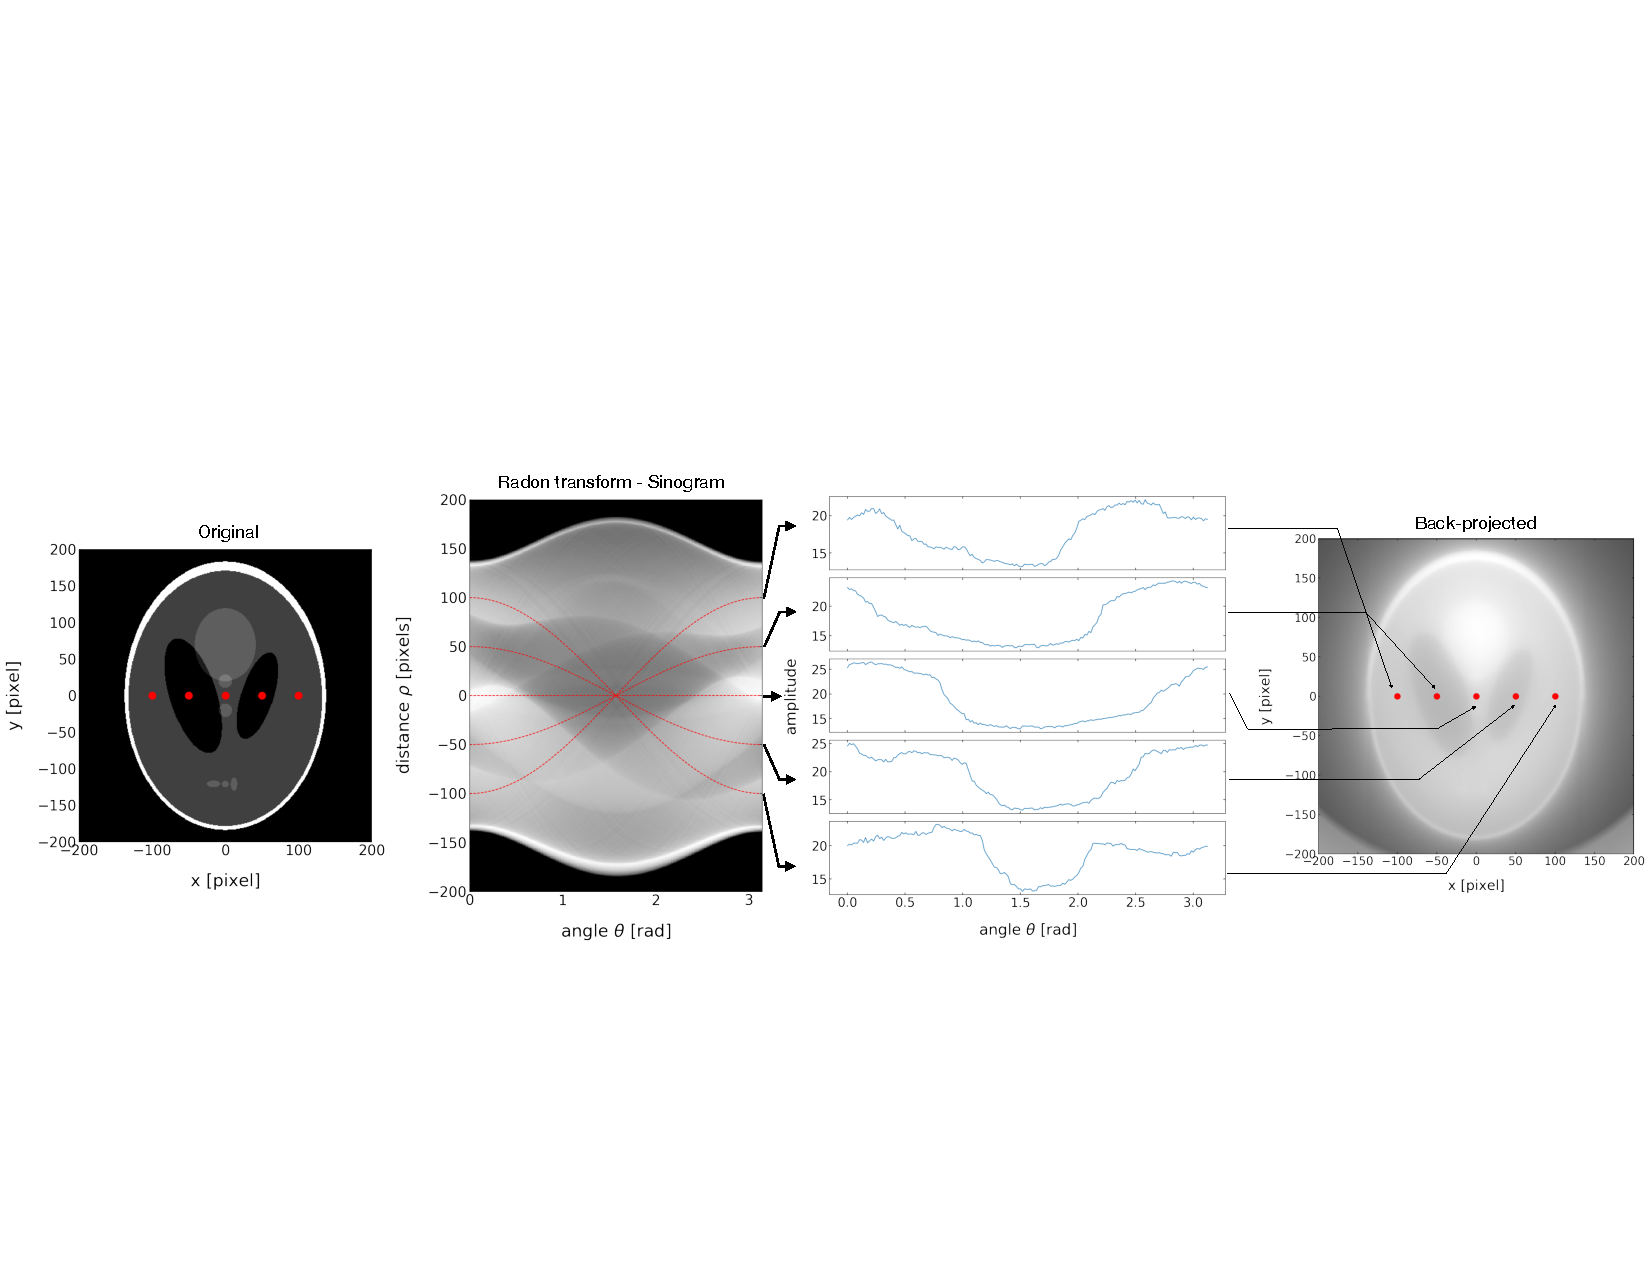
\includegraphics[width=1\textwidth]{inverse_radon/radon_transform.pdf}
	\caption{Original slice (left) and sinogram (middle) of the slice for the interval $\theta \in [0, \pi]$. The red dashed lines in the sinogram denote the information on the attenuation coefficients at the positions of the red dots in the original image. The intensity values of the sinogram along the red dashed lines are plotted in the right column. The integral over each of these curves deliver one value of one pixel in the reconstructed slice.}
\end{figure}

Employing eq. \ref{eq.12} we are able to back-project the Radon transform to compute a reconstructed slice. However, as I observed in Figure 7, no matter how many $\theta$ I back-project at, I will not be able to reconstruct the slice perfectly using the formula in eq. \ref{eq.13}. The back-projection results into a large amount of blurring, which will make fine details in heterogenous objects indistinguishable. I will therefore need to derive a method to filter our the noise the back-projection formula seems to create in our picture to obtain a more accurate reconstruction of the original slice. To arrive at this method I first have to introduce the Fourier Slice Theorem.
\subsubsection{Fourier Slice Theorem}
The Fourier Slice Theorem relates the two dimensional Fourier transform of $f(x,y)$ to the 1-dimensional Fourier transform of the Radon transform. I consider taking the projection of $f(x,y)$ at an angle $\theta_1$. Now I regard the 2-dimensional Fourier transform of the image, more specifically I inspect a slice in Fourier domain at the same angle $\theta_1$. This slice of the 2-dimensional Fourier transform is equal to the 1-dimensional Fourier transform of the projection as per Fourier Slice Theorem. I define the Fourier Slice Theorem mathematically as follows:
\begin{equation}\label{eq.14}
	\mathcal{F}[\breve{f}(\rho, \theta)](\nu) = \mathcal{F}_2[f(x,y)](\nu\cos{\theta}, \nu\sin{\theta})
\end{equation}
 The Fourier transform dissociates functions of time into its constituents frequencies. This makes it valuable when analysing all sort of signals. Similarly, the Fourier transform is also essential in image processing, as it dissociates the function of space into its spatial frequencies. In this specific case it bestows us with the relation between $f(x,y)$ and $\breve{f}(\rho, \theta)$. For this application of the Fourier transform I require only its basic properties. Therefore, I will not delve into detail about the Fourier transform as this is not necessary for this investigation and would solely complicate the comprehension of this matter. Nonetheless, I will derive the Fourier Slice Theorem which will significantly aid in the intricate understanding of the theorem. This will form a foundation of knowledge, such that I can introduce the filtered back-projection method.
 
 The 2-dimensional Fourier transform of $f(x,y)$ is given by
\begin{equation}\label{eq.15}
	\mathcal{F}_2(k_x, k_y) = \iint\limits_{\mathbb{R}^2} f(x,y)e^{-i(xk_x+ yk_y)} \, dx \, dy
\end{equation}
and relates the spatial distribution $f(x,y)$ to a distribution of spatial frequencies, $k_x$ and $k_y$, in the Fourier domain. The link to the Radon transform is not apparent in this form but will be readily obtained through a set of modifications. I first define the spatial frequencies $k_x$ and $k_y$, by polar form, in terms of $\theta$ and $\nu$, where $\theta \in [0, \pi]$ and $\nu \in \mathbb{R}$.
\begin{equation}\label{eq.16}
\begin{pmatrix} k_x \\ k_y \end{pmatrix} = \nu\begin{pmatrix} \cos{\theta} \\ \sin{\theta} \end{pmatrix}
\end{equation}
I substitute the spatial frequencies into eq. \ref{eq.15}
\begin{equation}\label{eq.17}
	\mathcal{F}_2(\nu\cos{\theta}, \nu\sin{\theta}) = \iint\limits_{\mathbb{R}^2} f(x,y)e^{-i\nu(x\cos{\theta} + y\cos{\theta})} \, dx \, dy
\end{equation}
By introducing the polar form I consider slices in the Fourier domain, rather than looking at the whole 2-dimensional Fourier transform of the $f(x,y)$. I then implement a change of variables from $x$ and $y$ to $\rho$ and $s$. This is obtained through the following correlations, which I defined when I parametrised the $L_{\rho, \theta}$.
\begin{equation}\label{eq.18}
	x = \rho\cos{\theta} - s\sin{\theta}, \, y = \rho\sin{\theta} + s\cos{\theta},\, \rho = x\cos{\theta} + y\sin{\theta}
\end{equation}
However, before changing the variables I first have to compute the determinant of the Jacobian for $x$ and $y$.
\begin{equation}\label{eq.19}
	\rm{det}\begin{vmatrix}
\frac{\partial x}{\partial \rho} & \frac{\partial x}{\partial s} \\
\frac{\partial y}{\partial \rho} & \frac{\partial y}{\partial s} \\
\end{vmatrix}
= 
\rm{det}\begin{vmatrix}
\cos{\theta} & -\sin{\theta} \\
\sin{\theta} & \cos{\theta} \\
\end{vmatrix}
= 1
\end{equation}
From the determinant I observe that $ds \,d\rho = dx \,dy$, such that I can rewrite eq. \ref{eq.17} as
\begin{equation}\label{eq.20}
	\mathcal{F}_2(\nu\cos{\theta}, \nu\sin{\theta}) = \iint\limits_{\mathbb{R}^2} f(\rho\cos{\theta}- s\sin{\theta}, \rho\sin{\theta} + s\cos{\theta}) e^{-i\nu\rho} \, ds \, d\rho 
\end{equation}
The right side of the equation almost appears to be equivalent to the Fourier transform of the Radon transform. Its equivalence is finally revealed through rearranging the differentials. Since $e^{-i\nu\rho}$ has no dependence on $s$ we can readily modify the integral in eq. \ref{eq.20} as follows:
\begin{equation}\label{eq.21}
	\mathcal{F}_2(\nu\cos{\theta}, \nu\sin{\theta}) = \int\limits_{\mathbb{R}}\left[\;\int\limits_{\mathbb{R}} f(\rho\cos{\theta}- s\sin{\theta}, \rho\sin{\theta} + s\cos{\theta})\, ds \right] e^{-i\nu\rho} \, d\rho 
\end{equation}
The inside of the bracket is identical to the  Radon transform $\breve{f}(\rho, \theta)$ as stated by eq. \ref{eq.11}, which implies that
\begin{equation}\label{eq:21}
	\mathcal{F}_2(\nu\cos{\theta}, \nu\sin{\theta}) = \int\limits_{\mathbb{R}} \breve{f}(\rho, \theta) e^{-i\nu\rho}\, d\rho
\end{equation}
This is the 1-dimensional Fourier transform of the Radon transform, with which I conclude the derivation of the Fourier Slice Theorem. I can therefore affirm the relationship of the $\breve{f}(\rho, \theta)$ and $f(x,y)$ which I acquire by employing the Fourier transform. 

This will form the basis of the filtered back-projection formula, which will be discussed in the following section.  

\subsubsection{Filtered Back-projection}
The filtered back-projection method is based on the Fourier Slice Theorem, to create a filtered transform that enhances the accuracy in the reconstruction of the original image.  
I look at the inverse 2-dimensional Fourier transform
\begin{equation}\label{eq.23}
	f(x,y) = \frac{1}{4\pi^2}\iint\limits_{\mathbb{R}^2} \mathcal{F}_2(k_x, k_y) e^{i(k_x x + k_y y)} dk_x dk_y
\end{equation}
and substitute eq. \ref{eq.16} into the inverse Fourier transform. I take the Jacobian determinant of eq. \ref{eq.16} to conduct a change of variables in the integral.
\begin{equation}\label{eq.24}
	\rm{det}\begin{vmatrix}
\frac{\partial k_x}{\partial \nu} & \frac{\partial k_x}{\partial \theta} \\
\frac{\partial k_y}{\partial \nu} & \frac{\partial k_y}{\partial \theta} \\
\end{vmatrix}
= 
\rm{det}\begin{vmatrix}
\cos{\theta} & -\nu\sin{\theta} \\
\sin{\theta} & \nu\cos{\theta} \\
\end{vmatrix}
= |\nu|
\end{equation}
This shows that $dk_x \, dk_y = |\nu|\,d\nu \,d\theta$. Incorporating the change in variables, I rewrite eq. \ref{eq.23} as
\begin{equation}\label{eq.25}
	f(x,y) = \frac{1}{4\pi^2}\int_{0}^{\pi} \int\limits_{\mathbb{R}}|\nu|\,\mathcal{F}_2(\nu\cos{\theta}, \nu\sin{\theta})\, e^{i\nu(x\cos{\theta}+y\sin{\theta}})\,d\nu\,d\theta
\end{equation}
Using the Fourier Slice Theorem in eq. \ref{eq.14} I can write eq. \ref{eq.25} as
\begin{equation}\label{eq.26}
	f(x,y) = \frac{1}{4\pi^2}\int_{0}^{\pi} \int\limits_{\mathbb{R}}|\nu|\,\mathcal{F}[\breve{f}(\rho, \theta)]\, e^{i\nu(x\cos{\theta}+y\sin{\theta})}\,d\nu\,d\theta
\end{equation}
This is the filtered back-projection formula. The 2-dimensional Fourier transform $\mathcal{F}_{2}$ has been replaced by the 1-dimensional Fourier transform $\mathcal{F}$ of the Radon transform with respect to $\rho$ with the help of the Fourier slice theorem. At the same time an additional factor $|\nu|$ occurs under the integral. This multiplier acts as a high-pass filter to the Radon transform, hence, filtered back-projection. A multiplication of two functions in Fourier space corresponds to a convolution of these functions in real space. Thus the Fourier transform of the Radon transform is convoluted with this function. Such a high-pass filter is characterised by its ability to suppress low frequencies while amplifying high frequencies. The $|\nu|$ filter performs this with linear function that is dependent on the frequency, illustrated in Figure 9.


Thus, with this filter, fine details (high-frequencies) are accentuated, while blurring (low-frequencies) is minimised. The form of the filtered back-projection which is displayed in eq. \ref{eq.26} is complicated and messy, therefore, I will simplify the formula. To achieve this I will first look at the inner integral by itself
\begin{equation}\label{eq.27}
	\int\limits_{\mathbb{R}}|\nu|\,\mathcal{F}[\breve{f}(\rho, \theta)]\, e^{i\nu(x\cos{\theta}+y\sin{\theta})}\,d\nu
\end{equation}
If I  rewrite the inner integral in a slightly different it becomes apparent that
\begin{align}
	 &= 2\pi\left(\frac{1}{2\pi}\int\limits_{\mathbb{R}}|\nu|\,\mathcal{F}[\breve{f}(\rho, \theta)]\, e^{i\nu(x\cos{\theta}+y\sin{\theta})}\,d\nu\right)\label{eq.28} \\
	&= 2\pi \, \mathcal{F}^{-1}[|\nu|\mathcal{F}\langle\breve{f}(\rho, \theta)\rangle](x\cos{\theta} + y\sin{\theta}, \theta)\label{eq.29}
\end{align}
the inner integral is $2\pi$ times the inverse Fourier transform of $|\nu|\breve{f}(\rho, \theta)$ at the point $(x\cos{\theta}+y\sin{\theta}, \theta)$. This allows me to rewrite eq. \ref{eq.26} as
\begin{equation}\label{eq.30}
	\frac{1}{2\pi}\int_{0}^{\pi} \mathcal{F}^{-1}[|\nu|\mathcal{F}\langle\breve{f}(\rho, \theta)\rangle](x\cos{\theta} + y\sin{\theta}, \theta)\, d\theta
\end{equation}
This relates to the initial back-projection formula in eq. \ref{eq.13} and is half the back-projection of $\mathcal{F}^{-1}[|\nu|\breve{f}(\rho, \theta)](x\cos{\theta} + y\sin{\theta}, \theta)$. I therefore simplify the above equation as
\begin{equation}\label{eq.31}
	f(x,y)=\frac{1}{2}\mathcal{B} \{ \mathcal{F}^{-1}[|\nu|\mathcal{F}\langle\breve{f}(\rho, \theta)\rangle](x\cos{\theta} + y\sin{\theta}, \theta) \}
\end{equation}
which is the desired form of the filtered back-projection. This method should allow us to reconstruct the original slice with higher accuracy. Figure \ref{fig:filtered_radon_transform} details the steps of the filtering process.
\begin{figure}[hbt]
	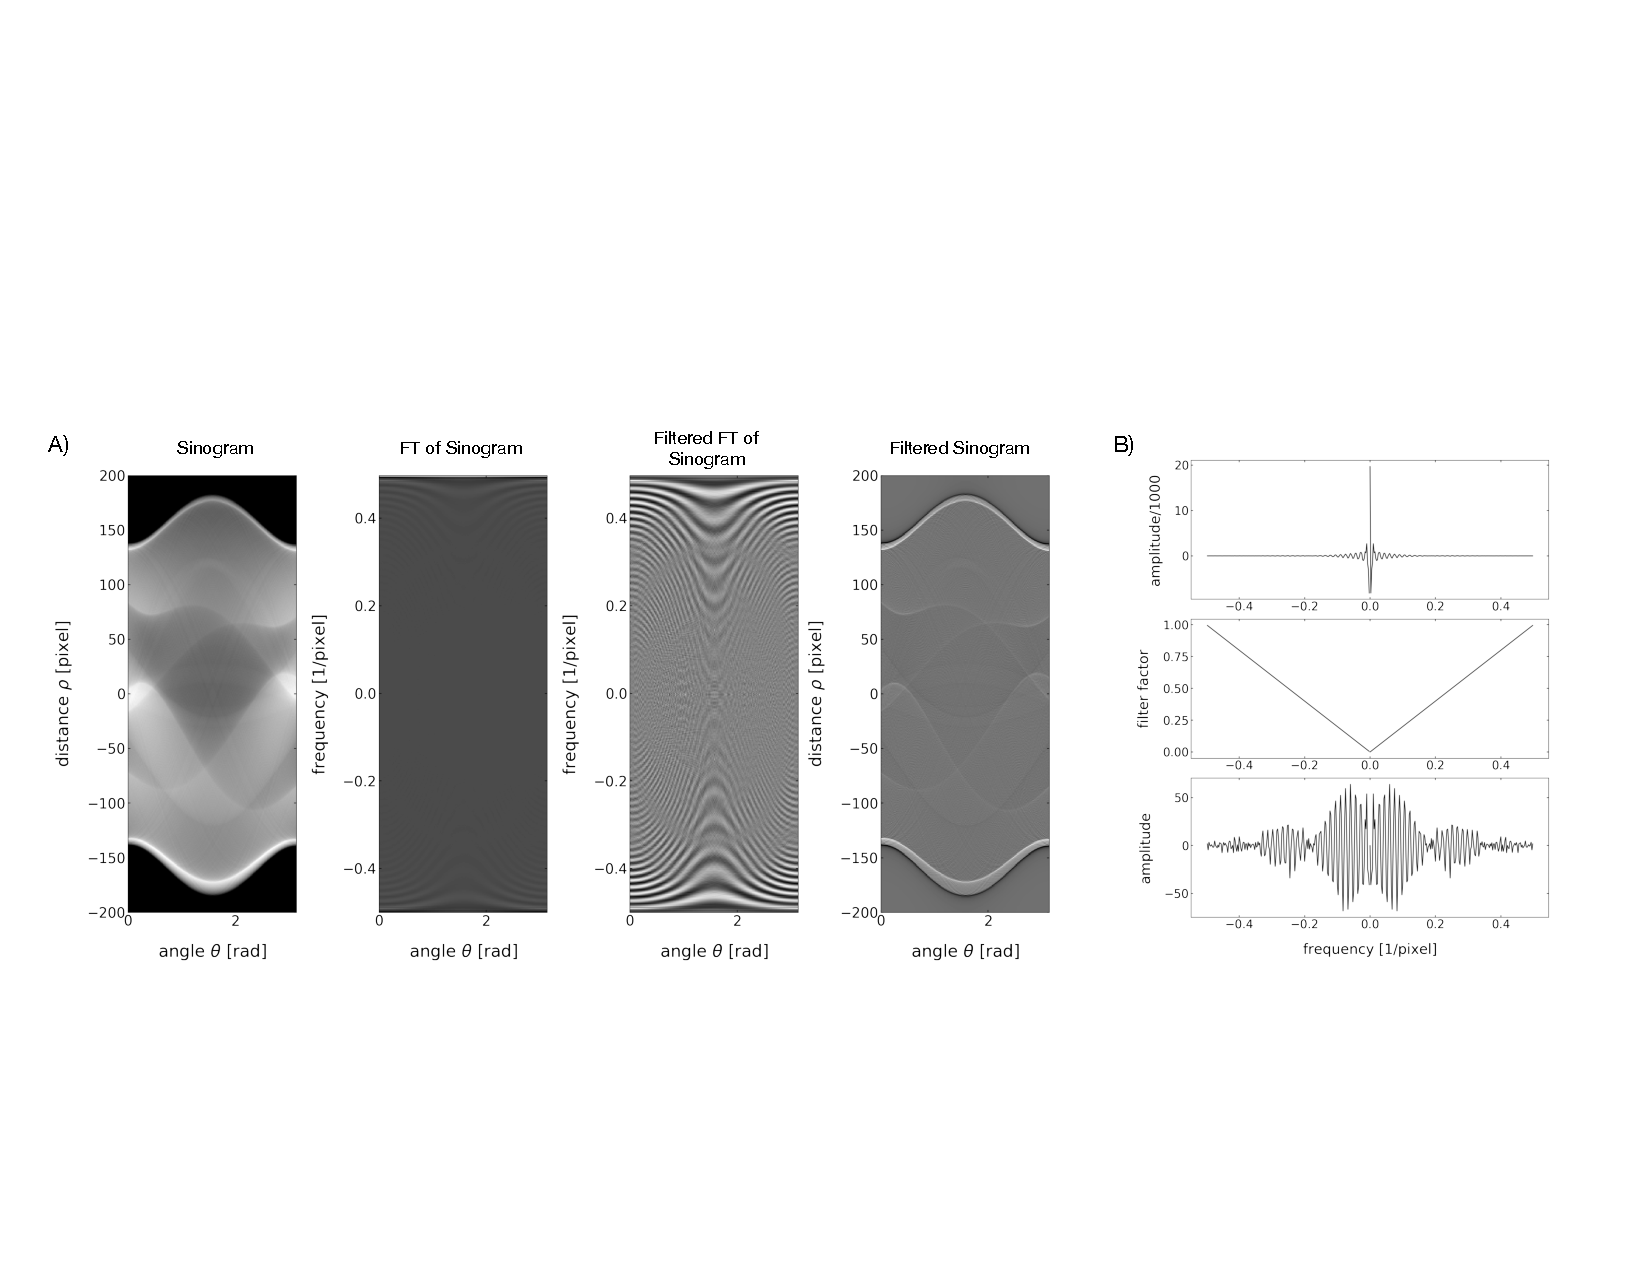
\includegraphics[width = 1\textwidth]{filtered/filtered_inverse_process.pdf}
	\caption{Filtering process of filtered back-projection method. A) illustrates the Fourier transform of the sinogram, the filtered Fourier transform of the sinogram and the filtered sinogram. B) portrays the application of the ramp filter on a slice of the Fourier transform of the sinogram}\label{fig:filtered_radon_transform}
\end{figure}
At first the sinogram is Fourier transformed along the $\rho$ coordinate for all angles $\theta$ (second column in Fig. \ref{fig:filtered_radon_transform} A). The Fourier transform is multiplied with the $|\nu|$ filter (so called ramp filter) for each angle (third column) and an inverse Fourier transform is applied to obtain the filtered sinogram. The graphs in Figure \ref{fig:filtered_radon_transform} B) highlight the change in the frequency spectrum for one column in the sinogram. The initial spectrum (top) is multiplied with the ramp filter (middle) to yield the filtered frequency spectrum (bottom).

Figure \ref{fig:inverse_filtered_radon_transform} displays the effect of the filtering as resulting from a self-written Python program following the above procedure. 

\begin{figure}[hbt]
	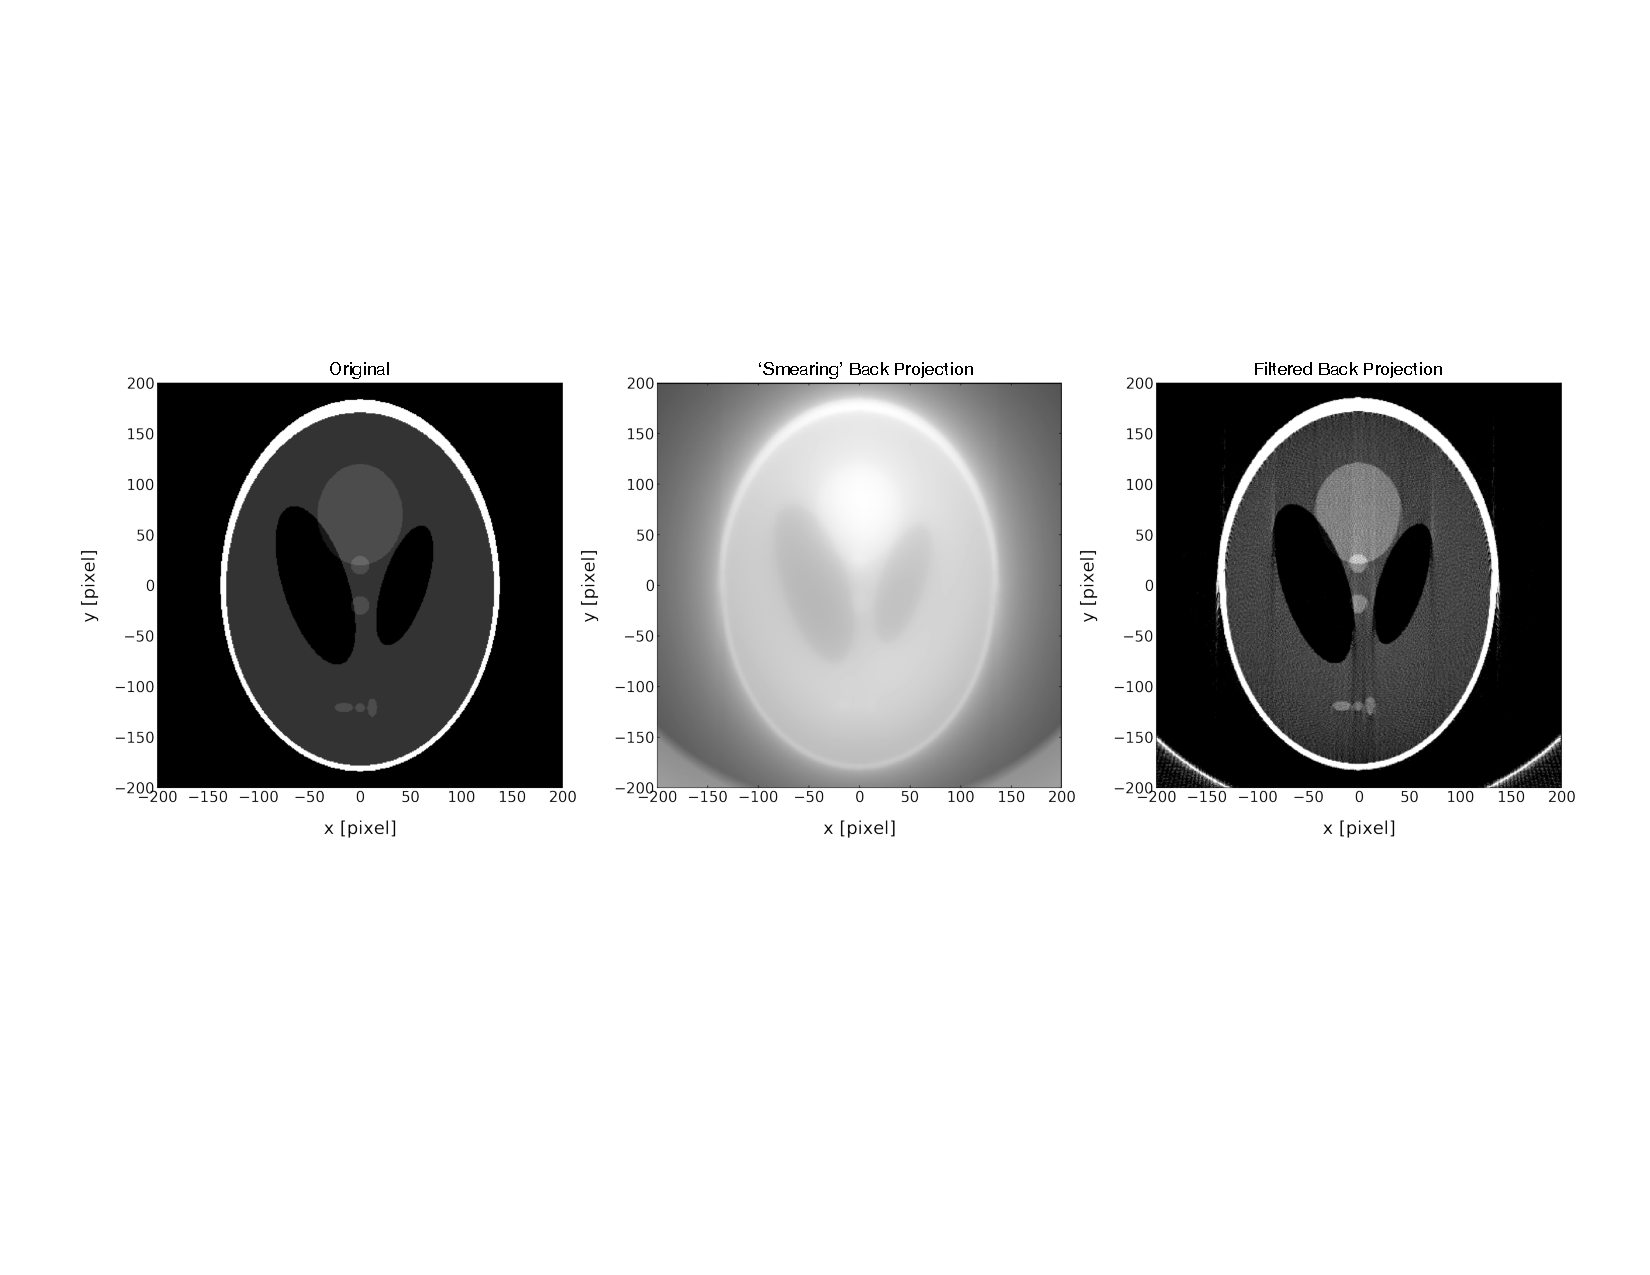
\includegraphics[width = 1\textwidth]{filtered/filtered_radon_transform.pdf}
	\caption{Reconstruction of the a sample slice ("Shepp-Logan Phantom"[9]) through filtered back-projection and 'smearing' back-projection.}\label{fig:inverse_filtered_radon_transform}
\end{figure}

The left image image in Figure \ref{fig:inverse_filtered_radon_transform} depicts the original slice, the middle image the result of the 'smearing' inverse Radon transform and the right image the resulting picture of the filtered inverse Fourier transform. Clearly, the self-written code still results in artefacts but gives considerably better results. To study the quality of the slice reconstruction  I will, however, refer to an implementation in the Python module 'skimage'[9].
%------------------------------------------------------------------------------------------------------------------------------------------------------------------------------------%
\section{Application}
Now that I have established two methods to reconstruct the original image from its projection. I will apply both reconstruction formulae on 3 different slices and perform an error calculation for the reconstructed slices. This should present a clear overview to the application of the Radon transform and its inverse in the field of medical imaging. Of course, in medical practices we have no original slice for comparison. Therefore, it is significant to evaluate the application of the reconstruction formula on  distinct slices as to ensure the accuracy of such a formula. I realised this through a python program (skimage module[9]), which first takes the Radon transform of the slice and then performs the filtered back-projection as well the 'smearing' back-projection to reconstruct the slice. The error of each back-projection formula was computed by calculating the difference between the original slice and the reconstructed slice. This yields an array of values from which I took the mean and root mean square (RMS) to determine the error of each method.

To characterise the deviation of the original slice from the reconstructed slice I define  $\Delta f(x_i,y_j)=f_{\rm slice}(x_i,y_j)-f_{\rm reconstructed}(x_i,y_j)$. Using this, the mean error can be calculated by

\begin{equation}\label{eq.mean}
	\rm{Mean} = \frac{1}{N^2}\sum\limits_{i=1}^{N} \sum \limits_{j=1}^{N}  \Delta f(x_i,y_j)
\end{equation}

where $N$ is the number of pixels per row and column. A second measure is the root mean squared error denoted by

\begin{equation}\label{eq.rms}
	\rm{RMS} =  \frac{1}{N}\sqrt{\sum\limits_{i=1}^{N} \sum \limits_{j=1}^{N}  \Delta f(x_i,y_j)^2}
\end{equation}

The latter is especially useful, when the values of $\Delta f(x_i,y_j)$ become positive and negative, such that they may cancel in the mean.

The results of the python program are illustrated in Figures \ref{fig.phantom}, \ref{fig.chess}, \ref{fig.landscape} and Table 1.
\begin{figure}[hbt]
	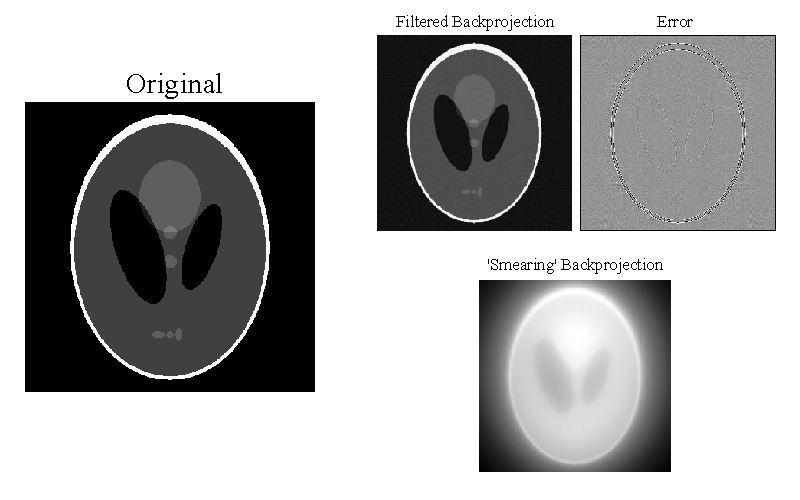
\includegraphics[width= .79\textwidth]{application/phantom}
	\caption{Reconstruction of "Shepp-Logan Phantom"[9] slice through filtered backprojection (eq. \ref{eq.31}) and 'smearing' backprojection (eq. \ref{eq.13}).}\label{fig.phantom}
\end{figure}
\begin{figure}[hbt]
	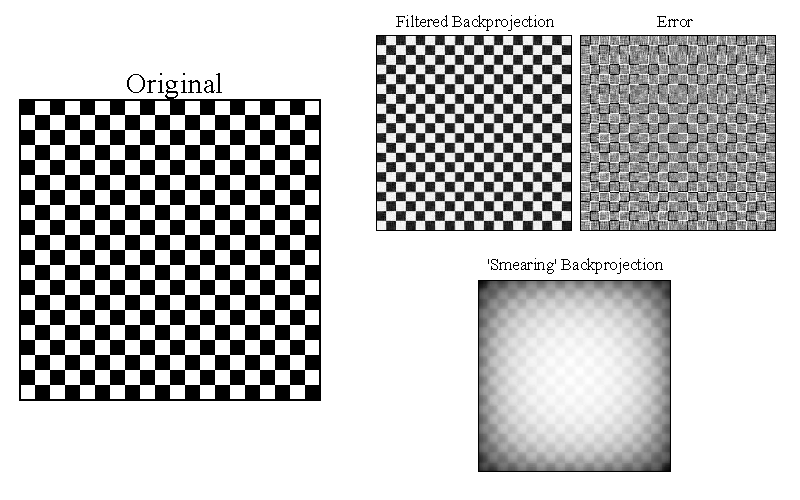
\includegraphics[width= .79\textwidth]{application/chess}
	\caption{Reconstruction of "chess board" slice through filtered backprojection (eq. \ref{eq.31}) and 'smearing' backprojection (eq. \ref{eq.13}).}\label{fig.chess}
\end{figure}
\clearpage
\vfill
\begin{figure}[hbt]
	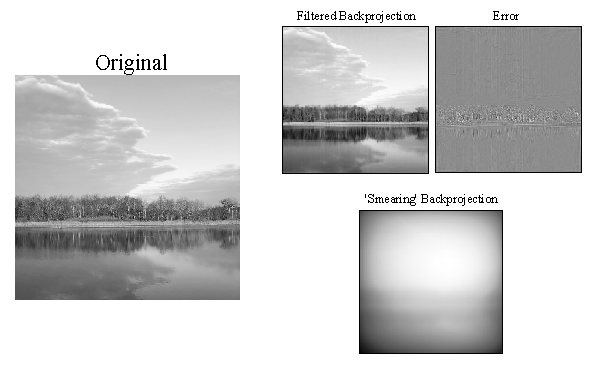
\includegraphics[width= \textwidth]{application/wildlife}
	\caption{Reconstruction of "landscape" slice through filtered back-projection (eq. \ref{eq.31}) and 'smearing' back-projection (eq. \ref{eq.13})}\label{fig.landscape}
\end{figure}
\vfill
\begin{table}[hbt]
    \caption{Error of reconstructed images. The values in the table have been obtained by employing eq. \ref{eq.mean} and eq. \ref{eq.rms}}
    \renewcommand{\arraystretch}{2.0}
    \label{tab:table1}
    \begin{tabularx}{\textwidth}{|X|>{\centering}X|>{\centering}X|>{\centering}X|>{\centering}X|}
    \hline
   		& \multicolumn{2}{c|}{\textbf{Filtered Back-projection}} & \multicolumn{2}{c|}{\textbf{'Smearing' Back-projection}}\tabularnewline
   		\cline{2-5}
        \textbf{\;\;\;\;\;\,Image} & Mean & RMS & Mean & RMS\tabularnewline
        \hline
      Shepp-Logan Phantom & -0.00247 & 0.0313 & 78.1& 80.9\tabularnewline
      \hline
      chess board & -0.0101 & 0.0865 & 297.& 299.\tabularnewline
      \hline
      landscape & -0.0127 & 0.0182 & 376. & 381.\tabularnewline
      \hline
    \end{tabularx}
\end{table}
\vfill
\clearpage
From equation eq. \ref{eq.31} we should expect that there the reconstructed slice is equal to the original slice. However, the python program employs the discrete Fourier transform instead of the continuous Fourier Transform that is used in eq. \ref{eq.31}. The results in an error in the reconstructed slice. When examining each Figure it becomes obvious that the filtered back-projection method performs much better than the 'smearing' back-projection in the reconstruction of the original slice. This observation is reflected by the error calculations shown in Table 1. I can also note that for an increase in the complexity of the slice the 'smearing' back-projection method performs drastically worse. For the "phantom" slice the error was calculated to be 80.9, however, the error for "chess board" slice rose distinctively, to 299; The "landscape" slice had an even higher error of 381. This conveys that for complex slice the 'smearing' back-projection formulae experiences a further decrease in the accuracy of the reconstructed slice. Contrastingly, the filtered back-projection performs at similar accuracy throughout all test slices. The "chess board" slice has given rise highest error for the RMS calculation but has the second highest error, when considering the mean. This is unexpected, since the trend, in the error of the 'smearing' back-projections, suggests that it be the second highest for the RMS and mean. I  require further analysis of the filtered back-projection formulae to justify this occurrence. 
\section{Discussion}
The understanding of the Fourier slice theorem might be assisted through the visual illustration of the reconstruction process. 
\begin{figure}[hbt]
	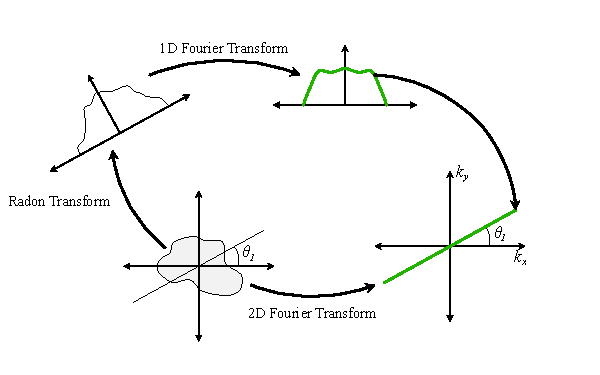
\includegraphics[width = .7\textwidth]{discussion/reconstruction_cycle}
	\caption{Slice reconstruction cycle. Relationship between the 1-dimensional Fourier transform of the Radon transform and the 2-dimensional Fourier transform of the slice.}\label{fig.recon}
\end{figure}
I will now investigate the reason for which the filtered back-projection is much more abundant in the accuracy of the reconstructed image in comparison to the 'smearing' back-projection.
Figure \ref{fig.recon} perfectly portrays that the 1-dimensional Fourier transform of a Radon transform at angle $\theta_1$ is equal to a slice of the 2-dimensional Fourier transform of the original image at the same angle. Accordingly, if I change the angle of projection, the angle at which I take the slice in the Fourier domain has to correspond to the equal angle. This already introduces us to the problem that arises from this method. Suppose I employ the Fourier Slice theorem to compute the reconstruct image from projection taken at a multitude of different angles. The resultant reconstructed slice would be similar to the original slice but would experience a large amount of blurring. This can be explained by the fact that, if we take multiple slices in Fourier domain at different angles, the area near the origin, the low-frequencies, are oversampled while the area farther from the origin, the high-frequencies, are under-sampled. In the Fourier domain instead of time frequencies (Hz) we have spatial frequencies. Spatial frequencies can be thought about as a grating of black and white bars; It is defined as the number of cycles in a grating within each degree of viewing angle.
\begin{figure}[hbt]
	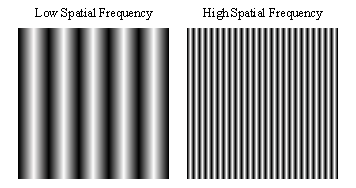
\includegraphics[width=.8\textwidth]{discussion/spatial_frequency}
	\caption{Spatial frequencies as a grating of black and white bar}\label{fig.freq}
\end{figure}

In Figure \ref{fig.freq} we observe that a low spatial frequency contains wide bars that are attributed with blurring. A grating with a high spatial frequency contains narrow bars that appear to be more defined. Subsequently, I deduce that low frequencies are the cause for the  blurring in the reconstructed image, and higher frequencies features the fine details. Therefore, to compute a more accurate reconstruction of the image we need the low frequencies to be minimised, instead of oversampled, and the high frequencies to be emphasised. It becomes obvious that we require a high-pass filter in the Fourier domain. The filter accentuates the high frequencies which makes finer details visible; It reduces the low frequencies to minimise the blurring in the reconstructed slice. This illustrates the reason explicably, why the filtered back-projection performs with a higher accuracy in comparison to the 'smearing' back-projection, which is most notable in complex slices.

However, I still have to address that the RMS error of the "chess board" is the highest while the mean error is the second highest. This can be explained by the fact that the "chess board" consists of a series of black and white squares, which have fine edges. In the Fourier domain these edges correspond to high spatial frequencies. When reconstructing the image we have an abundance of low frequencies due to the oversampling in the Fourier domain. Through the filter we are able to minimise the low frequencies and highlight high frequencies, however, the low frequencies cannot be eliminated fully which is the main cause for the error in the reconstruction. We therefore still experience minor blurring around the edges of the squares. The mean error of the reconstructed image is much lower than the RMS since the number of white and black squares are equal; The errors due to blurring, in this sense, cancel each other out. However, for the RMS the negative values we acquired when taking the difference between the reconstructed and the original image become positive, which results in the much larger error. 
\section{Conclusion}
I have researched the reconstruction of slices from its projections in the field of medical imaging. In medical imaging the projections of the slice at various angle $\theta$ is data that is acquired in a CT scanner, i.e. transmitting X-rays through the slice and recording the altered intensity with a detector. The first step to tackle this problem was to find a mathematical formula that would compute the projections of the slice, namely the Radon transform. I obtained a mathematical transform that mirrors the data acquisition performed in a CT scan. Subsequently, my investigation yielded two viable methods that act as an inversion formula to the Radon transform and allows the reconstruction of the original slice from its projections. The 'smearing' back-projection method is the more intuitive and apparent inversion formula. In non-mathematical terms the method can be considered as 'smearing' the projections onto the plane of the slice to reconstruct it. However, the reconstructed slice proved to have low accuracy when comparing it to the original slice. Therefore, I commenced my investigation of the more sophisticated filtered back-projection. This method employs a correlation between the original slice and its Radon transform that is given by the Fourier Slice Theorem. The ramp filter in the formula accentuates the fine details in the reconstructed slice and minimises blurring.  Through the application of both formulae I illustrated that the filtered back-projection performs with a much higher accuracy than the 'smearing' back-projection; And its suitability for reconstruction the original slice from its projections. As an outlook, I would like to mention that one could research the filter, which is employed in the filtered back-projection, more thoroughly to yield a filter that would enhance the accuracy of the reconstructed image even further.

\clearpage
\section{References}
\begin{enumerate}
	\item Beatty, Jen. The Radon Transform and the Mathematics of Medical Imaging.\\ 2012, digitalcommons.colby.edu/cgi/viewcontent.cgi?article=1649\&amp;\\context=honorstheses.
	\item Efford, Nick. “Spatial Frequency Domain.” Spatial Frequency Domain, www.cs.\\auckland.ac.nz/courses/compsci773s1c/lectures/ImageProcessing-html/topic1.htm.
	\item Fessler, J. Analytical Tomographic Image Reconstruction Methods. 2009, web.eecs.\\umich.edu/~fessler/course/516/l/c-tomo.pdf.
	\item Galt, James R., et al. “Filtering in Frequency Space.” Journal of Nuclear Medicine Technology, 1986, tech.snmjournals.org/content/14/3/152.full.pdf.
	\item “Image Processing.” Image Processing - MTH 337, www.math.buffalo.edu/~badzioch\\/MTH337/PT/PT-image\_processing/PT-image\_processing.html.
	\item Jørgensen, Jakob Sauer. “X-Ray Computed Tomography (CT).” 2008.
	\item Pan, Christine. “Backprojection Filters.” Backprojection Filters, 1996, www.clear.\\rice.edu/elec431/projects96/DSP/filters.html.
	\item Peters, Terry. “CT Image Reconstruction.” 2020, Robarts Research Institute, Robarts Research Institute.
	\item “Radon Transform.” Radon Transform - Skimage v0.17.dev0 Docs, scikit-image.org\\/docs/dev/auto\_examples/transform/plot\_radon\_transform.html.
	\item Stolk, Chris. The Radon Transform. 2014, pdfs.semanticscholar.org/3753/\\7e8a420b4892902f4a3858862b696128f7aa.pdf.
	\item Toft, Peter Aundal. “The Radon Transform/ Theory and Implementation.” Technical University of Denmark , 1996, pp. 95–96.
	\item Zisserman, A. “Lecture 2: 2D Fourier Transforms and Applications.” 2014.
	\item Zvolský, Milan. Tomographic Image Reconstruction. An Introduction. 2014, www.desy.de/~garutti/LECTURES/BioMedical/Lecture7\_ImageReconstruction.pdf.
\end{enumerate}
\end{document}

